\section{Estimación del SLA}
\label{sec:SLA}

El acrónimo \emph{SLA} corresponde a las siglas de \emph{Service Level
Agreement} o de Acuerdo de Nivel de Servicio. Este documento corresponde 
a un contrato entre el proveedor y un cliente para respaldar legalmente 
que el servicio cumple ciertos estándares de calidad concretos, como 
disponibilidad (\emph{uptime}), tiempo medio entre fallas (\emph{MTBF}),
tiempo medio de reposición de servicio (\emph{MTTR}), etcétera.

El \emph{SLA} es, en este caso, algo que se debe determinar a partir de 
las características del diseño del proyecto. Esto se debe a que existe 
una cierta infraestructura que será aprovechada para cumplir los 
objetivos buscados.

Entre los diversos elementos que permite garantizar el \emph{SLA} de
una red destacan:
\begin{itemize}
\item Servicios prestados
\item Parámetros de QoS:
  \begin{itemize}
  \item Throughput
  \item Ancho de banda medio
  \item Latencia máxima
  \item Interrupciones máximas
  \item Probabilidad de indisponibilidad de red
  \end{itemize}
\item Tarifas y facturación
\end{itemize}

Una forma en que puede variar el \emph{SLA} y que está considerado
entre las restricciones del proyecto es la probabilidad de cortes de
los cables.

\subsection{Modelo Probabilístico de la red}

La red de fibra oscura actual se compone de 6 data centers ubicados 
en la ciudad de Santiago y sus alrededores. La red posee cables de 
fibra oscura G.652.D que permiten el uso de 96 fibras ópticas en cada 
uno. Este tipo de fibra presenta una tasa de cortes anual de $0.05 
[\frac{\text{cortes}/\text{año}}{\text{km}}]$ en zona metropolitana y 
$0.01 [\frac{\text{cortes}/\text{año}}{\text{km}}]$ en zona rural. 
Debido a esto, es se espera que cada cierto tiempo, el camino que 
utilizaba la red para conectar un par de data centers esté 
inhabilitado y se requieran rutas alternativas con el fin de mantener 
un estándar de calidad en disponibilidad de conexión en la red.

Se define la probabilidad de que una conexión física (cable de fibra 
óptica G.652.D) entre 2 \emph{datacenters} separados por una distancia 
$L$, se encuentre inhabilitada por cierto periodo de tiempo $\Delta T$, 
como la probabilidad acumulada en el tiempo de $\Delta T$ (en días) 
según la tasa de corte anual por Km $R$ (en $\frac{\text{cortes}/\text{año}}{\text{km}}$) \eqref{proba_corte_1}.

\begin{equation}
\label{proba_corte_1}
P(\text{corte físico en }\Delta T) = L R \Delta T /365
\end{equation}

Luego se puede extender el concepto de conexión física entre dos 
\emph{datacenters} incluyendo los nodos de paso. La probabilidad de 
corte en este caso se calcula como el máximo de la probabilidad de 
corte de cualquiera de las conexiones entre los nodos pertenecientes al 
camino \eqref{proba_corte_2}.

\begin{equation}
\label{proba_corte_2}
P(\text{corte físico en }\Delta T) = \max_{i \in \text{Conexiones del Camino}} {L_i R_i \frac{\Delta T}{ 365}}
\end{equation}

El valor de esta probabilidad se puede reducir al agregar vías 
alternativas para conectar los dos \emph{datacenters}. Considerando 
independientes los sucesos que implican un corte en el cable, la 
probabilidad de indisponibilidad para la conexión entre ambos 
\emph{datacenters} será el producto de las probabilidades corte de cada 
camino \eqref{proba_corte_3}.

\begin{equation}
\label{proba_corte_3}
P(\text{indisponibilidad entre data centers A y B en }\Delta T) =  \prod_{j \in \text{Caminos}}\left( \frac{\Delta T}{365}\right) \max_{i \in \text{Conex. del Camino}} {L_{i,j} R_{i,j} }
\end{equation}

Dado que la tasa de cortes depende del tipo de zona en el que está 
inserto el \emph{datacenter}, la tasa de corte $R$ depende del camino 
que toma la conexión. Este modelo pretende establecer una estimación de 
la probabilidad de indisponibilidad de la conexión de cada par de 
\emph{datacenters}. Se escogió el periodo $\Delta T$ como el tiempo que 
los técnicos demoran en hacer las reparaciones en el corte de manera tal 
que la red vuelva a su estado normal. Este período se estima en torno a 
los 2 días como máximo según datos de referencia.

\subsection{Algortimo de cálculo de Conexiones}
\label{sec:algoritmo_conex}

La idea detrás de este algoritmo consiste en determinar un número fijo 
de vías de conexión entre cada par de \emph{datacenters} para cumplir 
con el \emph{SLA}. En otras palabras, se busca poder aseverar que la 
probabilidad de falla en la conexión entre dos \emph{datacenters} es 
menor a $0.01 \%$ dada una ventana de tiempo de 2 días, luego de la cual
se asume que esta falla será reparada.

Para obtener una red que sea capaz de cumplir con estos requerimientos 
se requiere que la expresión de la ecuación \eqref{proba_corte_3} esté 
acotada por este porcentaje ($0.01\%$). 

De esta forma, el algoritmo a utilizar es el siguiente: para cada par 
de \emph{datacenters} se procede de forma iterativa buscando los caminos 
que representan una menor distancia utilizando el algoritmo de Dijkstra
para optimización de grafos. Luego se calcula la probabilidad de corte 
\eqref{proba_corte_3} actual y la compara con el valor umbral. Si el 
valor umbral sigue siendo inferior, se remueve el último camino propuesto 
y se agrega el siguiente camino óptimo. Este proceso se repite hasta que 
se obtenga la probabilidad deseada o se acaben los caminos factibles.

Los resultados obtenidos por el algoritmo se muestran en la figura
\ref{fig:caminos}

\begin{figure}[H]
  \centering
  %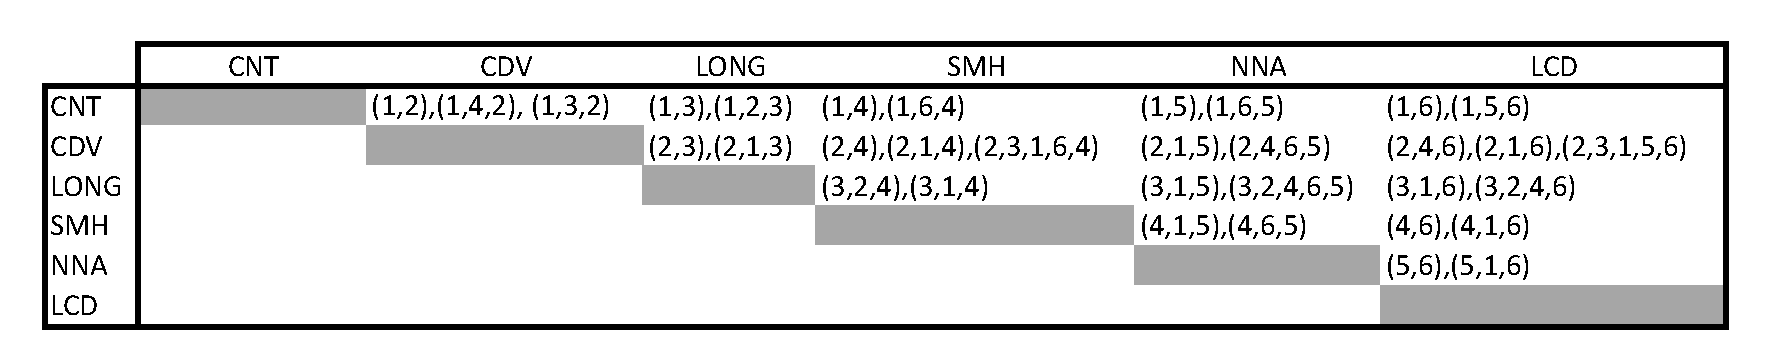
\includegraphics[width=13cm]{Imagenes/caminos}
  \caption{Caminos que pueden utilizar los datacenters para la comunicaciones, determinados según el algoritmo que fija la probabilidad de indisponibilidad.}
  \label{fig:caminos}
\end{figure}


\subsection{Efecto de la probabilidad de cortes de cable en el SLA}
\label{sec:cortes}

En una infraestructura de red oscura, un corte de cable entre dos data
centers significa que todas las conexiones entre esos data centers
quedan suspendidas hasta que los cables sean reparados físicamente
(introduciendo el valor \emph{MTTR}). Ello repercute directamente
en el \emph{SLA}, reduciendo el índice de interrupciones máximas.

Afortunadamente, el desarrollo actual permite acceder a la tecnología 
de conmutación dinámica de red ópticas de forma mucho más fácil
que hace algunos años. Acceder hoy a arquitecturas basadas en
\emph{WSON}, \emph{ROADM} y \emph{WSS} no aumenta significativamente el 
\emph{CAPEX}, \emph{OPEX} o la complejidad del proyecto, pero sí afecta 
sustancialmente al \emph{SLA}, introduciendo mejoras al índice de 
interrupciones máximas al reducir considerablemente el \emph{MTBF}.

Por otro lado, se pueden utilizar estimaciones de probabilidades de corte ...

\subsection{Garantías en cuanto al ancho de banda y \emph{throughput}
  de la red óptica}
\label{sec:anchodebanda}

Entre las especificaciones del proyecto, se pide un cierto número y
tipo de servicios para comunicaciones entre los \emph{datacenters}. Los
equipos instalados tras el diseño propuesto en este informe tienen la
obligación de dejar instalada la capacidad pedida en cada caso.

Las capacidades pedidas por \emph{datacenter} y por protocolo de
transmisión se muestran en las tablas \ref{tab:10ge} y \ref{tab:FC4G}.

\begin{table}[H]
  \centering
  \begin{tabular}{| l | c | c | c | c | c | c |}
    \hline
    \textbf{10GE} & \textbf{CNT} & \textbf{CDV} & \textbf{LONG} & \textbf{SMH} & \textbf{NNA} & \textbf{LCD} \\
    \hline
    \textbf{CNT}  & - & 20 & 10 & 4 & 4 & 6 \\
    \hline
    \textbf{CAD}  &   & - & 10 & 4 & 4 & 4 \\
    \hline
    \textbf{LONG} &   &   & - & 6 & 4 & 4 \\
    \hline
    \textbf{SMH}  &   &   &   & - & 4 & 4 \\
    \hline
    \textbf{NNA}  &   &   &   &   & - & 4 \\
    \hline
    \textbf{LCD}  &   &   &   &   &   & - \\
    \hline
  \end{tabular}
  \caption{Número de servicios entre data centers para protocolo 10GE}
  \label{tab:10ge}
\end{table}

 \begin{table}[H]
   \centering
   \begin{tabular}{| l | c | c | c | c | c | c |}
     \hline
     \textbf{FC 4G} & \textbf{CNT} & \textbf{CDV} & \textbf{LONG} & \textbf{SMH} & \textbf{NNA} & \textbf{LCD} \\
     \hline
     \textbf{CNT}  & - & 30 & 20 & 4 & 4 & 6 \\
     \hline
     \textbf{CAD}  &   & - & 20 & 4 & 4 & 4 \\
     \hline
     \textbf{LONG} &   &   & - & 6 & 4 & 4 \\
     \hline
     \textbf{SMH}  &   &   &   & - & 4 & 4 \\
     \hline
     \textbf{NNA}  &   &   &   &   & - & 4 \\
     \hline
     \textbf{LCD}  &   &   &   &   &   & - \\
     \hline
   \end{tabular}
   \caption{Número de servicios entre data centers para protocolo Fiber Channel 4G}
   \label{tab:FC4G}
 \end{table}
